\documentclass[11pt,english]{article}
\usepackage[T1]{fontenc}
\usepackage{fullpage}
\usepackage{babel}
\usepackage{graphicx}

\begin{document}

\title{\bf Real-Time Electronic Voting System}

\author{
    Marchand, Frederic \\
    \texttt{100xxxxxx}
    \and
    McBride, Tyler \\
    \texttt{100xxxxxx}
    \and
    Schurman, Brandon \\
    \texttt{100857068}
    \and
    Sikiru, Ibrahim \\
    \texttt{100xxxxxx}
}

\date{March 20, 2015}

\maketitle

In this project, we build an electronic version of the Canadian electoral system which is based
on a parliamentary system of government, modelled on that of the United Kingdom. The
people
in each electoral district vote for a candidate of their choice. The candidate who
receives the
most votes becomes Members of Parliament (MP) for that electoral district. After an election, the party with the most elected
representatives
becomes the party in power.


\section{System Architecture}

The Real-Time Electronic Voting System is programmed in Java as a distributed Client-Server
system. A number of Clients connect to servers which are representative of their local
electoral district. The Client systems are of a MVC architecture, and act as a polling
station for voters to register and vote once for their chosen candidate and party. The
client software allows voters to see the current statistics of the election in
real-time, and register and vote by validating with a local District Server. 
\vspace{2mm} \\
The District Servers processes all communication with the Clients in their district. They
store and validate the Client's registration, votes, and compute statistics on those
votes. A voter may only register through the Client once, and they need to login with the
server in order to vote. Once they have voted, the District Server will not allow
them to vote again.
\vspace{2mm} \\
The DistrictServers connect to a single CentralServer, which updates the entire federal election
results in soft real-time. The Central Server queries all of the District Servers
periodically for their current electoral statistics, and uses these statistics to compute
the results of the federal election. That is, it determines which party has the most votes
nation-wide. The system's distributed Client-Server architecture is depicted in
\underline{Figure 1.1} below. \\

\newpage 
\underline{Figure 1.1: The system architecture diagram} 
\vspace{5mm}\\
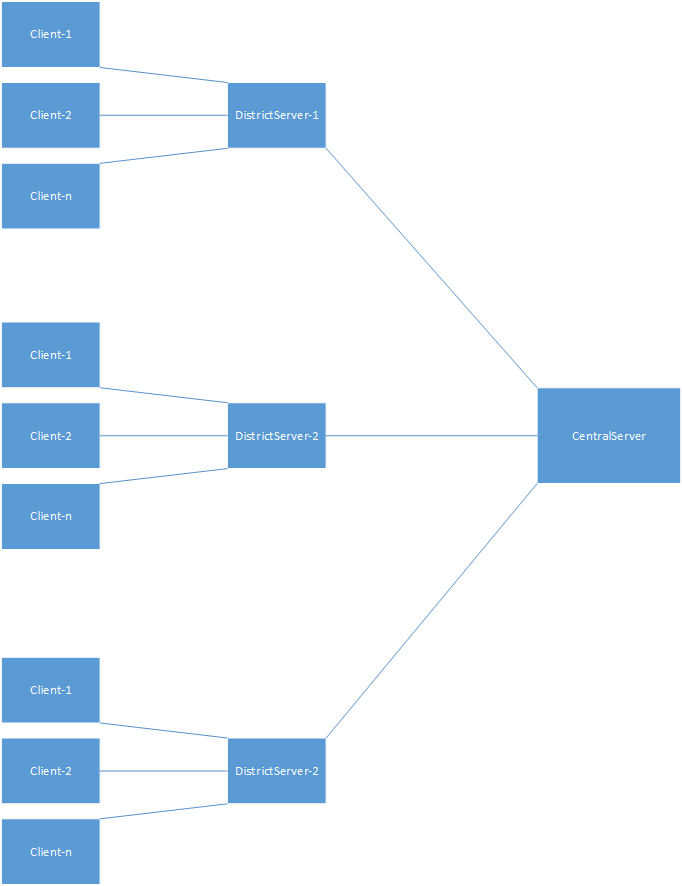
\includegraphics[width=6.2in]{figures/FlowChart.png}


\section{Java Class Implementation}

The System is implemented over a collection of Java classes, which are organized into Java
packages. The packages are {\tt controller}, {\tt model}, {\tt networking}, and {\tt
view}. The package organization corresponds to a typical Model-View-Controller design. The
classes contained within each package, and their relationships, are illustrated in the UML
class diagram found at \underline{Figure 2.1}. \\

\underline{Figure 2.1: UML class digarams}
\vspace{5mm}\\
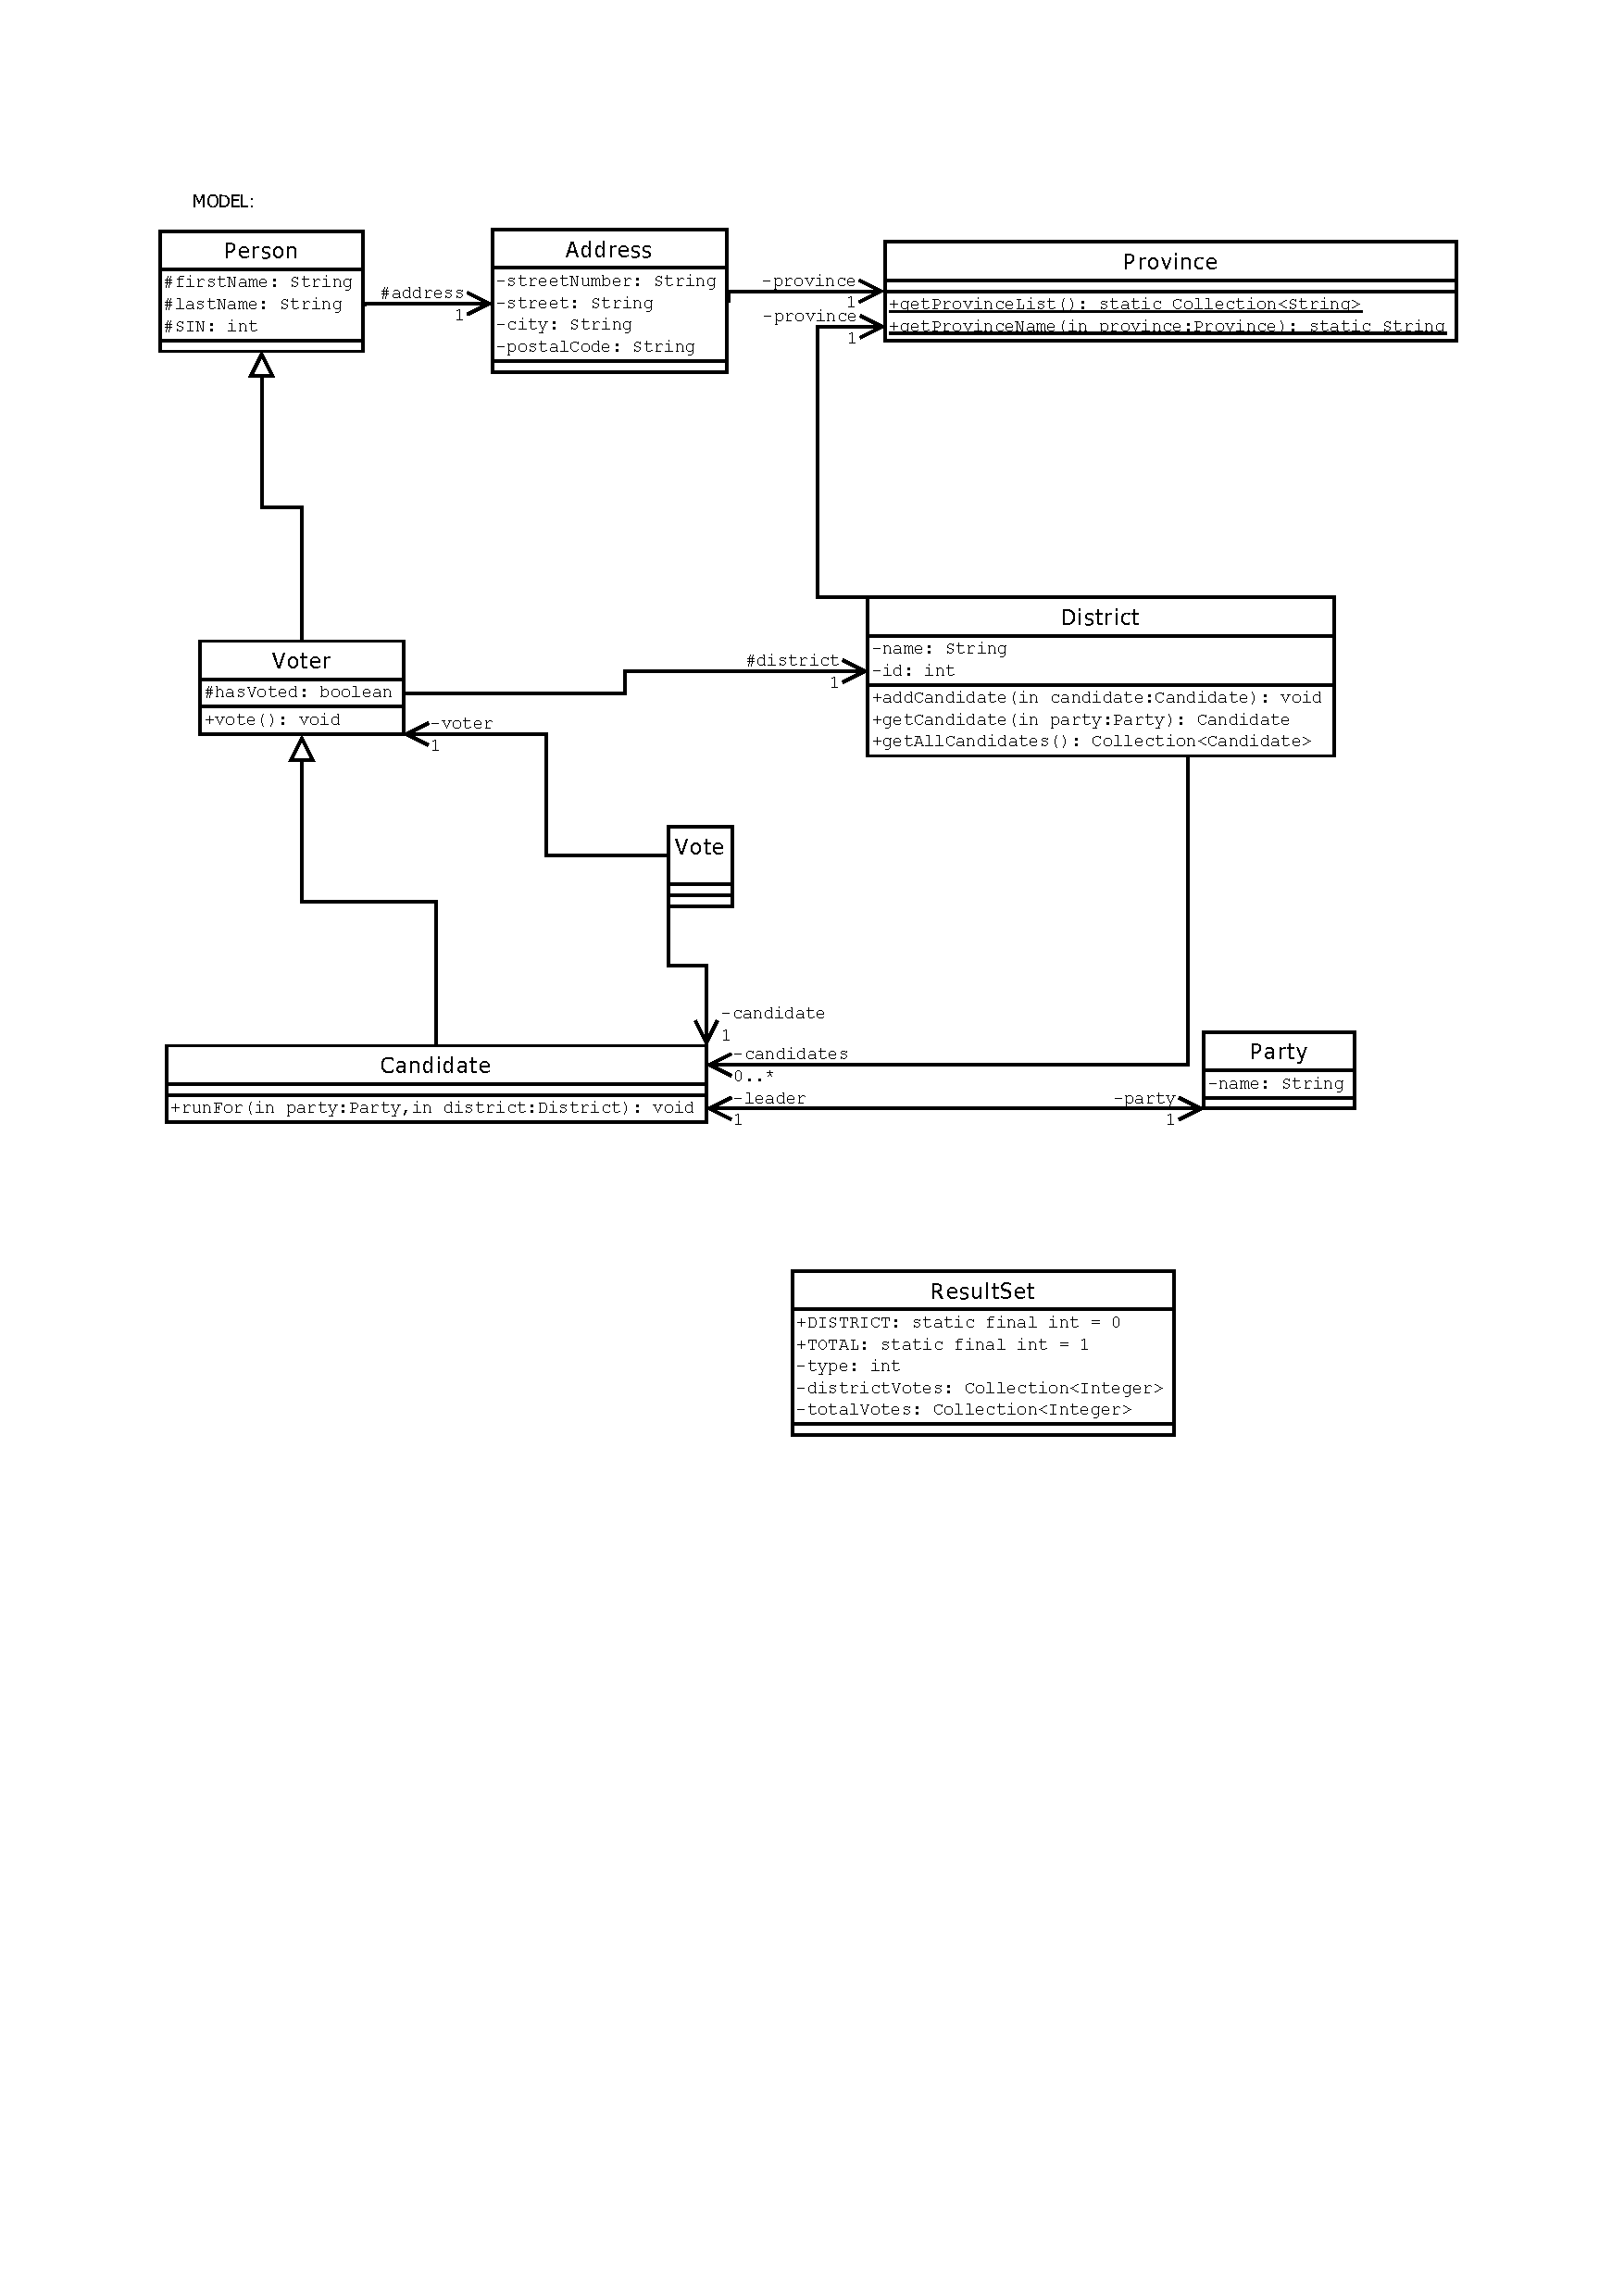
\includegraphics[width=4.5in]{figures/uml.pdf}


\section{The Communications Protocol}

The system's communication protocol is handled by a networking subsystem that
simulates the TCP protocol over a UDP connection. This networking component contains a
java class named, {\tt WSocket} (which stands for wrapper-socket). This class offers a
{\tt send} instance method which guarantees that message being passed are received by another
instance of {\tt WSocket}. It achieves this by sending a packet over a DatagramSocket, 
then waiting for another packet in response to signify that the data was received and intact. 
If no response is received, a {\tt TimeoutException} is thrown and the message is resent.
The {\tt WSocket}
class also offers a {\tt receive} method, which blocks and waits for a message to be received
over a datagram socket. When the message is received, it is deserialized and a CRC
checksum is calculated on the contained data. If the checksum indicates that the data is
corrupted, it does not send any notification message back to the sender. This effectively
causes the sender to resend the same message, since they will timeout after not receiving
a response. If the data is intact, a notification message is sent back to the sender and
the deserialized message is returned to the receiver. 
\vspace{2mm}\\
There is another limitation of using a UDP connection; and that is that individual packets
can only transport a small amount of data. The {\tt WSocket} class therefore breaks messages
that exceed the size of one packet into fragments. Fragments are sent and received in order,
following the same protocol outlined above, then are pieced back together by the receiver
to reconstruct the initial message. This protocol is illustrated in the two sequence
diagrams below. \underline{Figure 3.1} shows how the protocol operates for the sender,
which may be a Client in the Real-Time Electronic Voting System, and {\underline Figure
3.2} shows the protocol as it works for
the receiver, which may be a server in the system. Note that the exception handling, in
particular, for the timeout and message-corrupted exceptions, are not shown in these
diagrams.

\newpage
\underline{Figure 3.1: Sequence Diagram showing a sender's general usage of the socket} \\
\vspace{5mm}\\
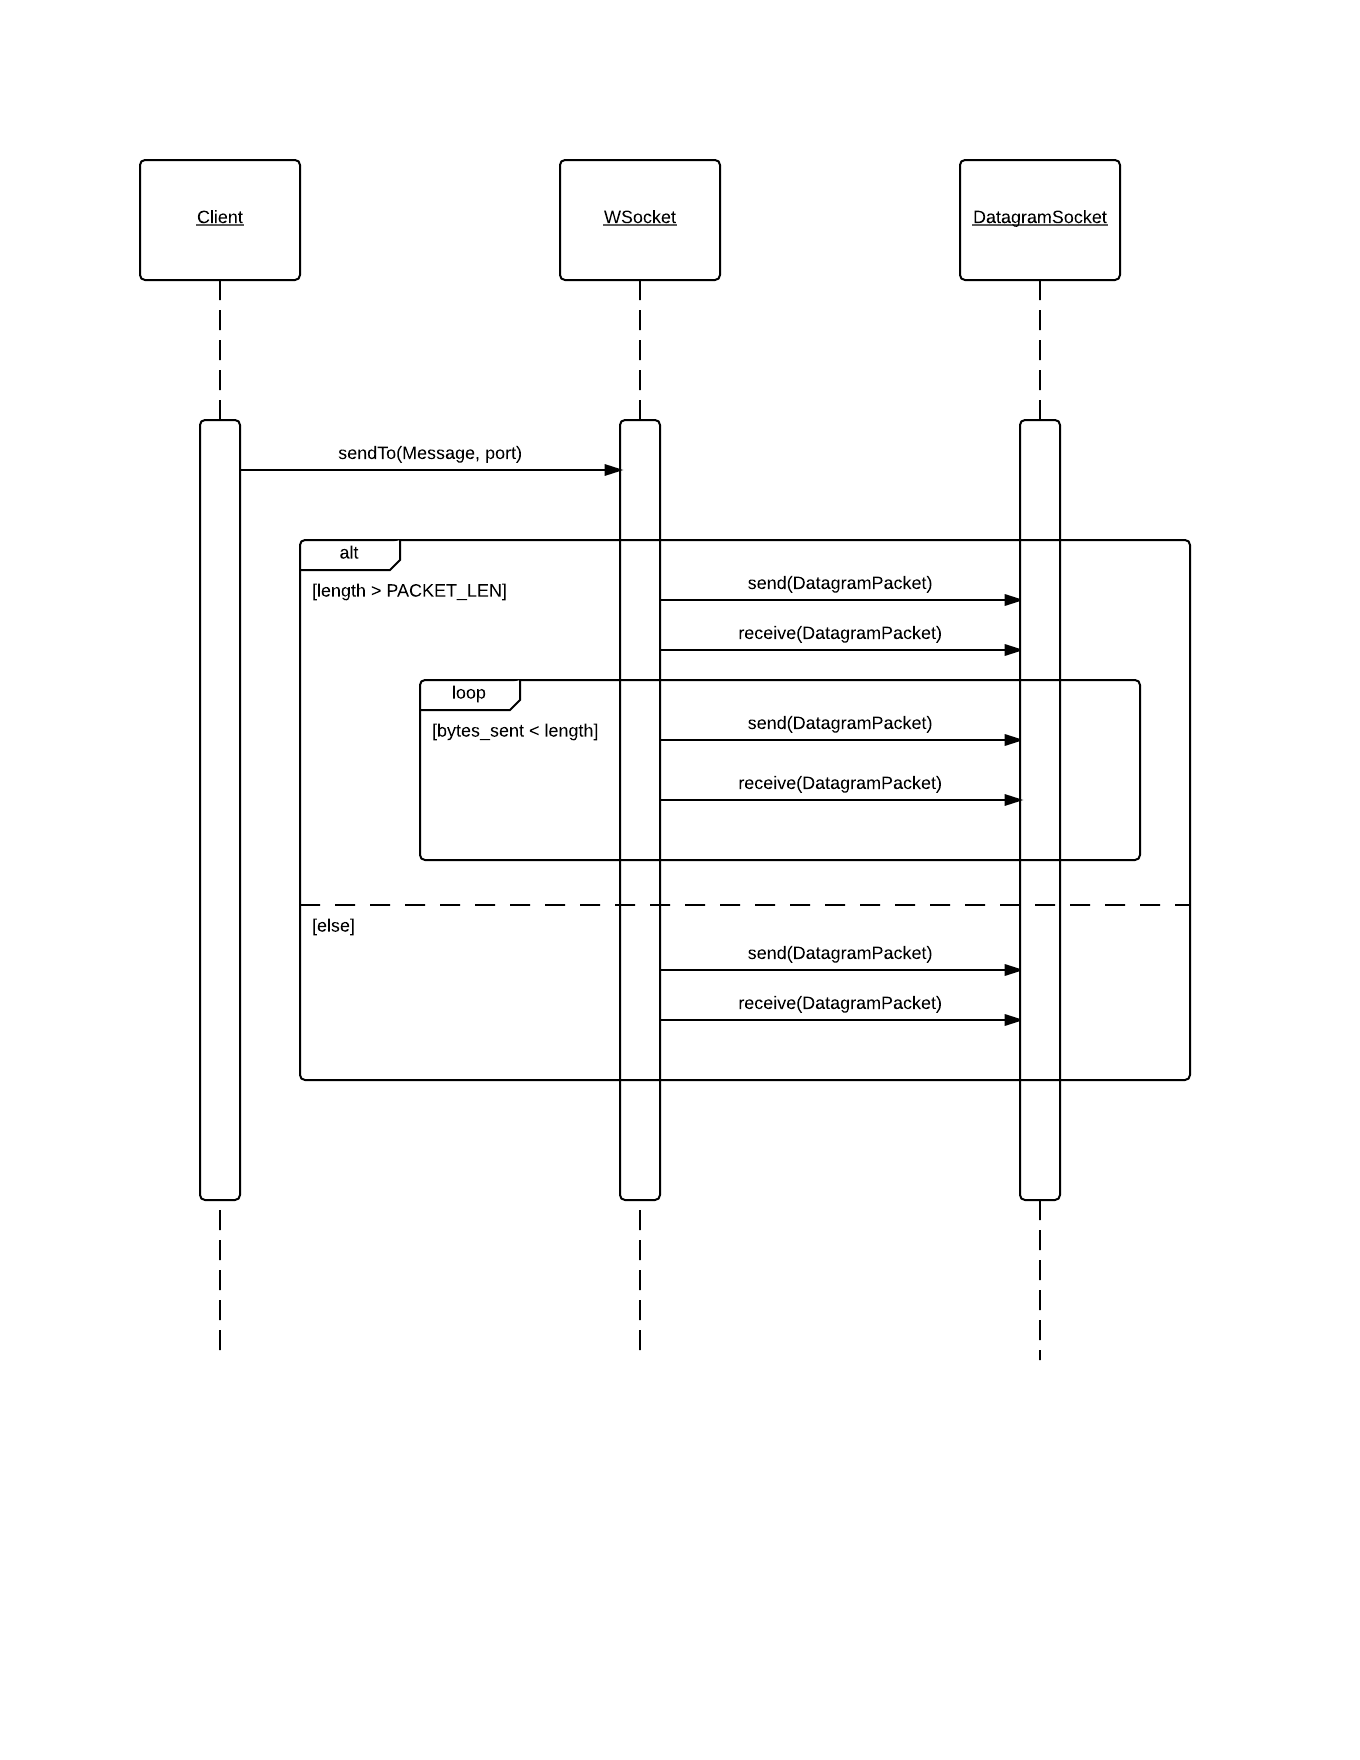
\includegraphics[width=6.2in]{figures/comm-protocol_seq-diagram_client.png}
\newpage
\underline{Figure 3.2: Sequence Diagram showing a receiver's general usage of the socket}
\vspace{5mm}\\
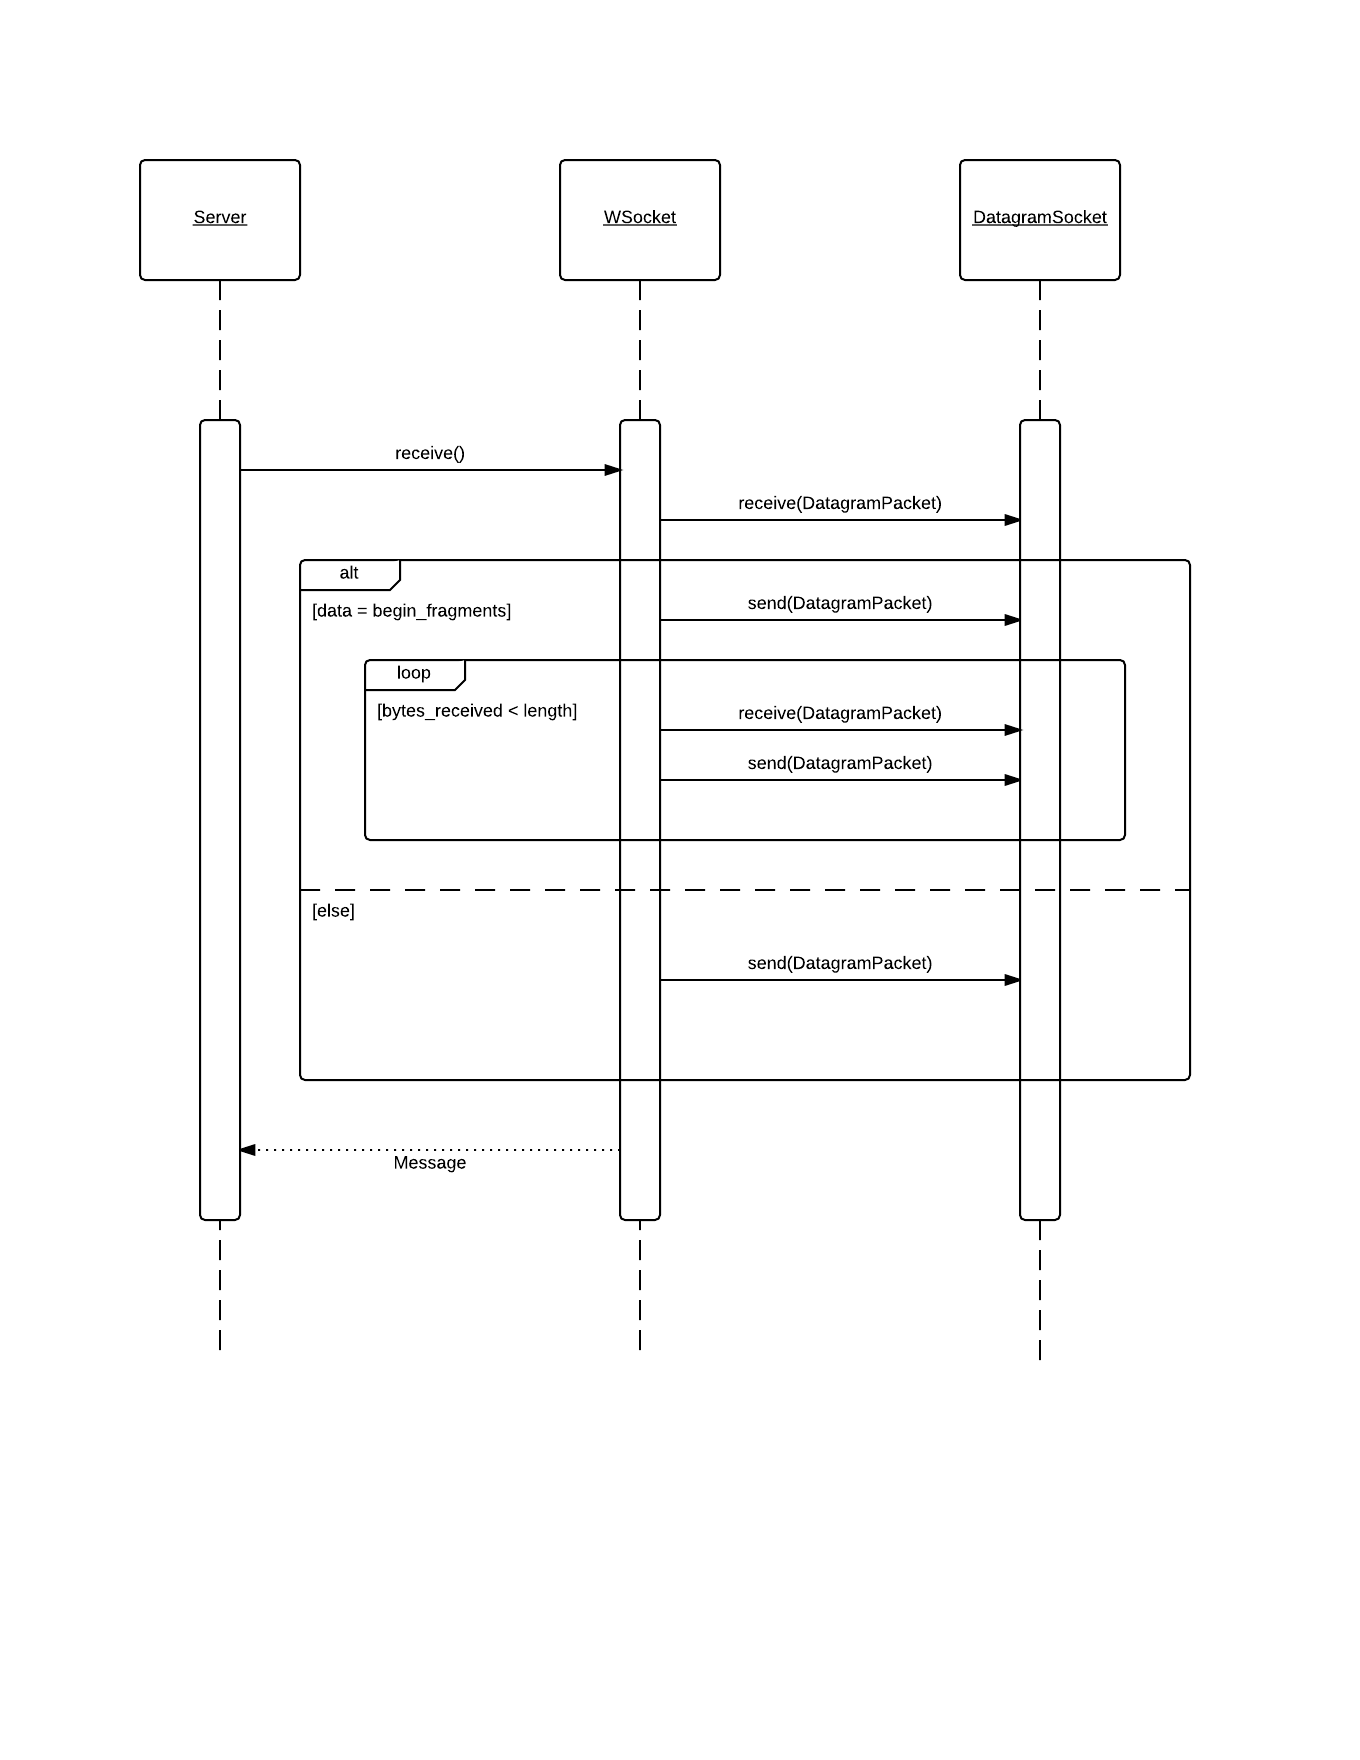
\includegraphics[width=6.2in]{figures/comm-protocol_seq-diagram_server.png}

\noindent More specifically, the Real-Time Electronic Voting System uses the networking subsystem to
send a finite set of message types. A typical interaction between a Client and District
Server may involve sending an odered sequence of messages. For example, a Client will
first request the list candidates running in that district. A voter may then
register with the District Server, then login, before they can send their vote.
Meanwhile, a background thread started by the Client periodically pings the current
election results from the server. This typical interaction is shown in the sequenec
diagram below. 
\vspace{10mm} \\
\underline{Figure 3.3: Typical message passing between a Client and the District Server}
\vspace{5mm}\\
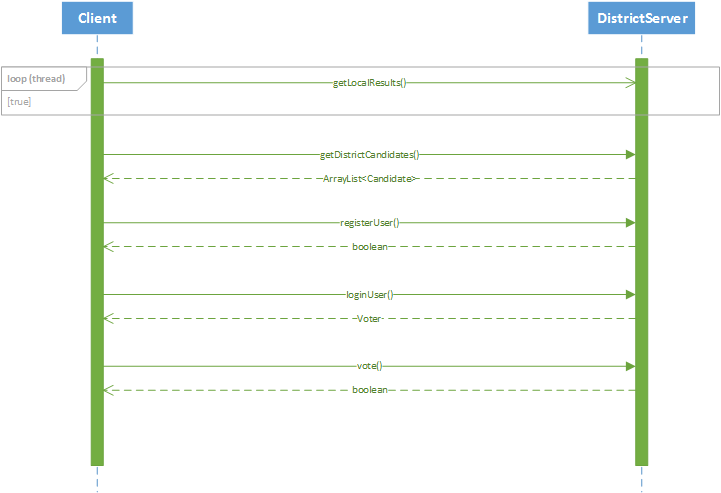
\includegraphics[width=7in]{figures/MSC.png}



\end{document}
